%
% LaTeX Problem Set Template by Sachin Padmanabhan
% I created this when I was a freshman in CS 103,
% and I continue to use it to this day.
%
% Hope you enjoy!
%
% There may be problems with this template.
% If so, feel free to contact me.
%

\documentclass[a4paper]{article}
\usepackage{amsmath}
\usepackage{amssymb}
\usepackage{amsthm}
\usepackage{amssymb}
\usepackage{mathdots}
\usepackage[pdftex]{graphicx}
\usepackage{fancyhdr}
\usepackage[margin=1in]{geometry}
\usepackage{multicol}
\usepackage{bm}
\usepackage{listings}
\PassOptionsToPackage{usenames,dvipsnames}{color}  %% Allow color names
\usepackage{pdfpages}
\usepackage{algpseudocode}
\usepackage{tikz}
\usepackage{enumitem}
\usepackage[T1]{fontenc}
\usepackage{inconsolata}
\usepackage{framed}
\usepackage{wasysym}
\usepackage[thinlines]{easytable}
\usepackage{hyperref}
\usepackage{dsfont}


\usepackage{wrapfig}
\setlength{\intextsep}{0pt}
\setlength{\columnsep}{0pt}
\usepackage{subcaption}
\usepackage{graphicx}
\graphicspath{ {images/} }

\hypersetup{
    colorlinks=true,
    linkcolor=blue,
    filecolor=magenta,
    urlcolor=blue,
}

\title{
\textsc{Iran university of science and technology} \\ [25pt] % Your university, school and/or department name(s)
Discrete mathematics\\Problem Set \#2 \\
}
\author{Ali Heydari}
\date{\today}

\lhead{Ali Heydari}
\chead{Problem Set \#2}
\rhead{\today}
\lfoot{}
\cfoot{Discrete mathematics --- Winter 2018}
\rfoot{\thepage}

\newcommand{\abs}[1]{\lvert #1 \rvert}
\newcommand{\absfit}[1]{\left\lvert #1 \right\rvert}
\newcommand{\norm}[1]{\left\lVert #1 \right\rVert}
\newcommand{\eval}[3]{\left[#1\right]_{#2}^{#3}}
\renewcommand{\(}{\left(}
\renewcommand{\)}{\right)}
\newcommand{\floor}[1]{\left\lfloor#1\right\rfloor}
\newcommand{\ceil}[1]{\left\lceil#1\right\rceil}
\newcommand{\pd}[1]{\frac{\partial}{\partial #1}}
\newcommand{\inner}[1]{\langle#1\rangle}
\newcommand{\cond}{\bigg|}
\newcommand{\rank}[1]{\mathbf{rank}(#1)}
\newcommand{\range}[1]{\mathbf{range}(#1)}
\newcommand{\nullsp}[1]{\mathbf{null}(#1)}
\newcommand{\repr}[1]{\left\langle#1\right\rangle}

\DeclareMathOperator{\Var}{Var}
\DeclareMathOperator{\tr}{tr}
\DeclareMathOperator{\Tr}{\mathbf{Tr}}
\DeclareMathOperator{\diag}{\mathbf{diag}}
\DeclareMathOperator{\dist}{\mathbf{dist}}
\DeclareMathOperator{\prob}{\mathbf{prob}}
\DeclareMathOperator{\dom}{\mathbf{dom}}
\DeclareMathOperator{\E}{\mathbf{E}}
\DeclareMathOperator{\R}{\mathbb{R}}
\DeclareMathOperator{\var}{\mathbf{var}}
\DeclareMathOperator{\quartile}{\mathbf{quartile}}
\DeclareMathOperator{\conv}{\mathbf{conv}}
\DeclareMathOperator{\VC}{VC}
\DeclareMathOperator*{\argmax}{arg\,max}
\DeclareMathOperator*{\argmin}{arg\,min}
\DeclareMathOperator{\Ber}{Bernoulli}
\DeclareMathOperator{\NP}{\mathbf{NP}}
\DeclareMathOperator{\coNP}{\mathbf{coNP}}
\DeclareMathOperator{\TIME}{\mathsf{TIME}}
\DeclareMathOperator{\polytime}{\mathbf{P}}
\DeclareMathOperator{\PH}{\mathbf{PH}}
\DeclareMathOperator{\SIZE}{\mathbf{SIZE}}
\DeclareMathOperator{\ATIME}{\mathbf{ATIME}}
\DeclareMathOperator{\SPACE}{\mathbf{SPACE}}
\DeclareMathOperator{\ASPACE}{\mathbf{ASPACE}}
\DeclareMathOperator{\NSPACE}{\mathbf{NSPACE}}
\DeclareMathOperator{\Z}{\mathbb{Z}}
\DeclareMathOperator{\N}{\mathbb{N}}
\DeclareMathOperator{\EXP}{\mathbf{EXP}}
\DeclareMathOperator{\NEXP}{\mathbf{NEXP}}
\DeclareMathOperator{\NTIME}{\mathbf{NTIME}}
\DeclareMathOperator{\DTIME}{\mathbf{DTIME}}
\DeclareMathOperator{\poly}{poly}
\DeclareMathOperator{\BPP}{\mathbf{BPP}}
\DeclareMathOperator{\ZPP}{\mathbf{ZPP}}
\DeclareMathOperator{\RP}{\mathbf{RP}}
\DeclareMathOperator{\coRP}{\mathbf{coRP}}
\DeclareMathOperator{\BPL}{\mathbf{BPL}}
\DeclareMathOperator{\IP}{\mathbf{IP}}
\DeclareMathOperator{\PSPACE}{\mathbf{PSPACE}}
\DeclareMathOperator{\NPSPACE}{\mathbf{NPSPACE}}
\DeclareMathOperator{\SAT}{\mathsf{SAT}}
\DeclareMathOperator{\NL}{\mathbf{NL}}
\DeclareMathOperator{\PCP}{\mathbf{PCP}}
\DeclareMathOperator{\PP}{\mathbf{PP}}
\DeclareMathOperator{\cost}{cost}
\let\Pr\relax
\DeclareMathOperator*{\Pr}{\mathbf{Pr}}

\definecolor{shadecolor}{gray}{0.95}

\theoremstyle{plain}
\newtheorem*{lem}{Lemma}

\theoremstyle{plain}
\newtheorem*{claim}{Claim}

\theoremstyle{definition}
\newtheorem*{answer}{Answer}

\newtheorem{theorem}{Theorem}[section]
\newtheorem*{thm}{Theorem}
\newtheorem{corollary}{Corollary}[theorem]
\newtheorem{lemma}[theorem]{Lemma}

\renewcommand{\headrulewidth}{0.4pt}
\renewcommand{\footrulewidth}{0.4pt}

\setlength{\parindent}{0pt}

\pagestyle{fancy}

\renewcommand{\thefootnote}{\fnsymbol{footnote}}

\begin{document}

\maketitle

\section{Two Is Irrational?}

In lecture, we proved that $\sqrt{2}$ is irrational, and in the checkpoint problem you proved that $\sqrt{3}$ is irrational.
Below is a purported proof that $\sqrt{4}$ is irrational:

\begin{theorem}
  $\sqrt{4}$  is irrational.
\end{theorem}
\begin{proof}
  Assume for the sake of contradiction that $\sqrt{4}$ is rational. Then there must exist
integers $p$ and $q$ where $ q \neq 0 $, where $p / q = \sqrt{4}$ , and where $p$ and $q$ have no
common factors other than $1$ and$ -1$.
Since $p / q = \sqrt{4}$ , we have $p^2 / q^2 = 4$, so $p^2 = 4q^2$. Since $q^2$ is an integer, we see
that $p^2$ is a multiple of four, and therefore $p$ is a multiple of four. Thus $p = 4n$
for some integer $n$.
Since $4q^2 = p^2$ and $p = 4n$, we have $4q^2 = (4n)^2 = 16n^2$, so $q^2 = 4n^2$. Since $n^2$ is an
integer, we see that $q^2$ is a multiple of four, so $q$ is a multiple of four as well.
But since both $p$ and $q$ are multiples of four, we see that $p$ and $q$ share a common
divisor other than $1$ and $-1$, contradicting our initial assumption. We have
reached a contradiction, so our assumption must have been incorrect. Thus $\sqrt{4}$
is irrational.
\end{proof}
This proof has to be wrong, because$ \sqrt{4} = 2 = 2/1$, which is indeed rational!
What error does this proof make that lets it conclude $\sqrt{4}$ is irrational? Why doesn't this error occur
in the similar proofs that $\sqrt{2}$ and $\sqrt{3}$ are irrational?
\begin{shaded}
\begin{answer}
Just because $p^2$ is divisible by $4$, that doesn't mean $p$ is.
\end{answer}
\end{shaded}

\section{Modular Arithmetic}
Many different numbers yield the same remainder when divided by some number. For example, the
numbers $2, 5, 8, 11, 14$, and $17$, all leave a remainder of two when divided by three, while the numbers
$1, 12, 23, 34,$ and $45$ all leave a remainder of one when divided by eleven. To formalize this relationship
between numbers, we'll introduce a relation $ \equiv_k $  that, intuitively, indicates that two numbers
leave the same remainder when divided by $k$. For example, we'd say that $1 \equiv_{11} 12 $ and that $8 \equiv_3 11$.

\begin{enumerate}[label*=\roman*.,ref=\roman*]
\item Prove that for any integer $x$ and any integer $x$ that $ x \equiv_k x $.
\begin{shaded}
\begin{answer}
\begin{proof}
 $$ \forall x \in \mathds{Z} \quad : \quad k | x - x \quad \Rightarrow \quad x \equiv_k x $$
\end{proof}
\end{answer}
\end{shaded}

\item Prove that for any integers $x$ and $y$ and any integer $k$ that if $x \equiv_k y$, then $y \equiv_k x$.
\begin{shaded}
\begin{answer}
\begin{proof}
$$ \forall x , y \in \mathds{Z} $$
\begin{equation}\label{x , y mod k}
x \equiv_k y \quad \Rightarrow \quad k | x - y
\end{equation}
\begin{equation}\label{x - y = y - x}
  k | x - y \quad = \quad k | y - x
\end{equation}
$$ \text{from} \quad \ref{x - y = y - x}, \ref{x , y mod k} \quad \Rightarrow \quad y \equiv_k x $$
\end{proof}
\end{answer}
\end{shaded}

\item Prove that for any integers $x, y$, and $z$ and any integer $k$ that if $x \equiv_k y$ and $y \equiv_k z$, then $x \equiv_k z$.
\begin{shaded}
\begin{answer}
\begin{proof}
$$ \forall x , y , x \in \mathds{Z} $$
\begin{equation}\label{y , z mod k}
  y \equiv_k z \quad \Rightarrow \quad k | y - z
\end{equation}
$$ \text{from} \quad \ref{x , y mod k} , \ref{y , z mod k} \quad \Rightarrow \quad k | x - z \quad \Rightarrow x \equiv_k z  $$
\end{proof}
\end{answer}
\end{shaded}


\end{enumerate}
\section{Pigeonhole Principle 1}
\paragraph*{
There are 51 senators in a senate. The senate needs to be divided into $n$ committees such that each senator is on exactly one committee. Each senator hates exactly three other senators.(If senator $A$ hates senator $B$, then senator $B$ does $’not'$ necessarily hate senator $A$.)
}
\paragraph*{
Find the smallest $n$ such that it is always possible to arrange the committees so that no senator hates another senator on his or her committee.
}
\begin{shaded}
\begin{answer}
\begin{proof}
In the worst case, consider that senator $S$ hates a set of 3 senators, while he himself is hated by a completely different set of 3 other senators. Thus, given one senator, there may be a maximum of 6 other senators whom he cannot work with. If we have a minimum of 7 committees, there should be at least one committee suitable for the senator $S$ after the assignment of the 6 conflicting senators.
\end{proof}
\end{answer}
\end{shaded}

\section{Pigeonhole Principle 2}
Let $\Omega$ be a set of points in the plane. Each point in $\Omega$ is a midpoint of two points in $\Omega$ . Show that $\Omega$ is an infinite set.
\begin{shaded}
\begin{answer}

Fist proof:
\begin{proof}
Suppose $\Omega$ is a finite set. Then $\Omega$ contains two points $A, B$ with
maximal distance $|AB|  = m $. $B$ is a midpoint of some segment $C $ $ D $ with $C$, $ D  \in \Omega $.
Figure.
\ref{Problem4Fig1}
 shows that $ |AC| > |AB|$ or $|AD| > |AB|$.
\end{proof}


\begin{proof}
We consider all points in $\Omega$ farthest to the left, and among those
the point $M$ farthest down. $M$ cannot be a midpoint of two points $A,B \in \Omega $ since
one element of $\{A,B\}$ would be either left of $M$ or on the vertical below $M$.
\end{proof}
\end{answer}
\end{shaded}

\begin{figure}[h]
\centering
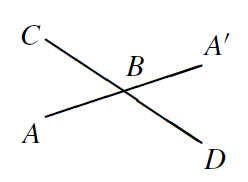
\includegraphics{Problem4Fig1}
\caption{}\label{Problem4Fig1}
\end{figure}

\section{Pigeonhole Principle 3}
A plain is colored blue  and red in any way. prove that there exists a rectangle with vertices of same color.

\begin{shaded}
\begin{answer}
\begin{proof}
Choose any 7 collinear points. At least 4 of these points are of the same color, say
red. Call them $ R_1, R_2, R_3, R_4 $. We project these points onto two lines parallel to the
first line to $S_1, \dots , S_4 $ and $T_1, \dots , T_4$. If two S-points or two T -points are red, then
we have a red rectangle. Otherwise, there exist 3 blue S-points and 3 T -points, and
hence, a blue rectangle.
\end{proof}
\end{answer}
\end{shaded}

\section{Pigeonhole Principle 4}
Prove that having 100 whole numbers, one can choose 15 of them so that the difference of any two is divisible by 7
\begin{shaded}
\begin{proof}
For the difference to be a multiple of 7, the integers must have equal modulo 7 residues. To avoid having 15 with the same residue, 14 numbers with different modulo 7 residues can be picked ($14 * 7 = 98$). Thus, two numbers are left over and have to share a modulo 7 residue with the other numbers under the pigeonhole principle.
\end{proof}
\end{shaded}

\section{Contradiction every where}
$2n + 1$ persons are placed in the plane so their mutual distances are all distinct. Then everyone
shoots his nearest neighbor. Prove that (a) at least one person survives (b) nobody is hit by more than
5 bullets (c) the set of segments formed by the bullet paths does not contain a closed polygon.
\begin{shaded}
\begin{answer}
$$  $$
\begin{proof}
(a) All mutual distances are different. Hence there exist two persons $A$ and $B$ with
minimum distance. These two persons will shoot each other. If any other person
shoots at $A$ or $B$, someone will survive since $A$ and $B$ have used up three bullets. If
not, we can ignore $A$ and $B$. We are left with the same problem with n replaced by
$n − 1$. Repeating the argument, we either find a pair at whom three shots are fired,
or if not, we arrive, finally, at three persons, and for this case $(n = 1)$, the theorem
is obvious.
\end{proof}
\begin{proof}
(b) Suppose the persons $A,B,C,D, . . . $ shoot at $P$ (Figure. \ref{Problem7Fig1}). $A$ shoots at $P$ and
not at $B$, so $|AP| < |AB|$. $B$ shoots at $P$ and not at $A$, so $|BP| < |AB|$. Thus, $AB$ is
the largest side in the triangle $A\,B\,P$. The largest angle lies opposite the largest side.
Hence, $\gamma > \alpha, \gamma > \beta$ or $2\gamma > \alpha + \beta, 3\gamma > \alpha + \beta + \gamma ,\gamma > 60^{\circ}$. Thus any two
bullet paths meeting at $P$ make an angle greater than $60^{\circ}$. Since $6 \times 60^{\circ}  = 360^{\circ}$,
five bullet paths at most can meet at $P$.

\end{proof}
\begin{proof}
(c) Suppose the paths of two bullets cross with $A$ shooting at $B$ and $C$ shooting
at $D$ (Figure. \ref{Problem7Fig2}). Then $|AB| < |AD|$ and $|CD| < |CB|\quad $ imply $\quad |AB| + |CD| <
|AD| + |CB|$. On the other hand, by the triangle inequality, \\  $ \quad |AS| + |SD| > |AD| \quad $
and $ \quad |BS| + |SC| > |BC| \quad \Rightarrow \quad |AB| + |CD| > |AD| + |BC|$. Contradiction!
\end{proof}
\begin{proof}
  (d) Suppose there is a closed polygon $ABCDE \dots  MN$  (Figure. \ref{Problem7Fig3}) . Let $|AN| <
|AB|$, that is, $N$ is the nearest neighbor of $A$. Then $|AB| < |BC|, |BC| < |CD|,
|CD| < |DE|, . . ., |MN| < |NA|$, that is, $|AB| < |NA|$. Contradiction! The
assumption $|AN| > |AB|$ also leads to a contradiction.
\end{proof}
\end{answer}
\end{shaded}
\begin{figure}[h]
  \centering
\begin{subfigure}{0.45\textwidth}
\centering
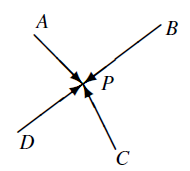
\includegraphics[scale = 0.7]{Problem7Fig1}
\caption{}\label{Problem7Fig1}
\end{subfigure}

\begin{subfigure}{0.45\textwidth}
\centering
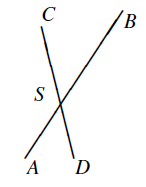
\includegraphics[scale = 0.7]{Problem7Fig2}
\caption{}\label{Problem7Fig2}
\end{subfigure}
\begin{subfigure}{0.45\textwidth}
\centering
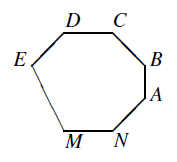
\includegraphics[scale = 0.7]{Problem7Fig3}
\caption{}\label{Problem7Fig3}
\end{subfigure}
\caption{} \label{Problem7 Figures}
\end{figure}


\end{document} 